\begin{Exercise}[title=trois chats et un triangle]
  Trois chats se trouvent initialement aux sommets d'un triangle équilatéral. Ils se poursuivent les uns les autres : le premier court après le second qui poursuit le troisième, lui même courant après le premier. Leur vitesse est la même et reste constante au cours de la poursuite.
\Question Déterminer la durée de la poursuite.
\Question En déduire la distance parcourue par chacun des chats.
\Question Déterminer l'équation de la trajectoire d'un des chats en coordonnées polaires.
\end{Exercise}
\begin{Answer}
  \begin{center}
    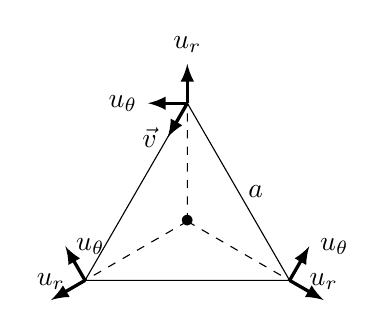
\begin{tikzpicture}[scale=0.5]
      \draw[dashed] (0,0)node{$\bullet$} -- (90:3)
      (0,0) -- (210:3)
      (0,0) -- (-30:3);
      \draw
      (90:3) -- (210:3) --(-30:3) --(90:3) node[midway,right]{$a$};

      \draw[very thick,-latex] (90:3) -- ++(240:1) node[left]{$\vec{v}$};
      \draw[very thick,-latex](90:3) -- ++ (-1,0) node[left]{$u_\theta$};
      \draw[very thick,-latex](90:3) -- ++ (0,1) node[above]{$u_r$};
      \draw[very thick,-latex](210:3) -- ++ (120:1) node[right]{$u_\theta$};
      \draw[very thick,-latex](210:3) -- ++(210:1) node[above]{$u_r$};
      \draw[very thick,-latex](-30:3) -- ++ (60:1) node[right]{$u_\theta$};
      \draw[very thick,-latex](-30:3) -- ++ (-30:1) node[above]{$u_r$};
    \end{tikzpicture}
  \end{center}

  \Question Le problème est invariant par rotation et par mise à l'échelle. $r_0= \sqrt{3} a$
  \[ \vec{v} =
    \begin{pmatrix}
      -\sin \frac{\pi}{3}\\
      \cos \frac{\pi}{3}
   \end{pmatrix}v =
      \begin{pmatrix}
-1/\sqrt{2} \\  1/2
\end{pmatrix} v =
\begin{pmatrix}
\dot{r} \\ r\dot{\theta}
\end{pmatrix}
\implies
\begin{cases}
  r = -\frac{v t}{\sqrt{2}}+r_0 \\
  \theta = \frac{1}{\sqrt{2}} \ln\left(\frac{vt}{\sqrt{2}}+r_0\right)
\end{cases}
\]
\Question les chats se rencontre en $r=0$ à $t=\sqrt{6}\frac{a}{v}$.
\Question les chats ont une vitesse constante donc $d= vt_0 =\sqrt{6}a$
\end{Answer}
